\documentclass[11pt]{article}

\usepackage[margin=1in]{geometry}
\usepackage{parskip}
\usepackage{amsmath,amssymb,amsthm}
\usepackage{tikz}
\usetikzlibrary{arrows.meta}
\tikzset{lbl/.style={draw=none, fill=none, minimum size=0pt,
  inner sep=1pt, font=\scriptsize}}

\pagestyle{plain}

\begin{document}

\begin{center}
  {\large \textbf{MATH 5810 Spring 2025}} \\[4pt]
  {\large \textbf{Worksheet: Flows and Cuts}}
\end{center}

\medskip
\noindent\rule{\textwidth}{0.4pt}

$c$ : capacity function, \quad $f$ : flow function, \quad
$s$ : source, \quad $t$ : sink, \quad $E(G)$ : the arc set of $G$

The \textbf{value} of $f$, denoted $v(f)$, is defined as the
net flow out of $s$.

A flow $f$ satisfies: (1) $0 \le f(uv) \le c(uv)$ for all
$uv \in E(G)$, and (2) at every node except $s$ and $t$,
flow in $=$ flow out.

\noindent\rule{\textwidth}{0.4pt}

\bigskip

% =====================================================================
% PROBLEM 1
% =====================================================================
\textbf{Problem 1.}
Consider the network below with flow/capacity labels $f/c$ on
each edge.

\begin{center}
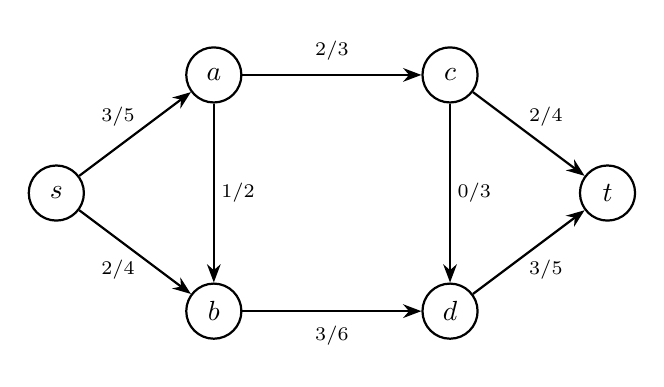
\begin{tikzpicture}[every node/.style={circle, draw, minimum size=7mm,
  inner sep=0pt}, >=Stealth, thick]
  \node (s) at (0, 0)   {$s$};
  \node (a) at (2, 1.5)  {$a$};
  \node (b) at (2, -1.5) {$b$};
  \node (c) at (5, 1.5)  {$c$};
  \node (d) at (5, -1.5) {$d$};
  \node (t) at (7, 0)   {$t$};
  \draw[->] (s) -- node[lbl, above left]  {$3/5$} (a);
  \draw[->] (s) -- node[lbl, below left]  {$2/4$} (b);
  \draw[->] (a) -- node[lbl, above]       {$2/3$} (c);
  \draw[->] (a) -- node[lbl, right]       {$1/2$} (b);
  \draw[->] (b) -- node[lbl, below]       {$3/6$} (d);
  \draw[->] (c) -- node[lbl, above right] {$2/4$} (t);
  \draw[->] (c) -- node[lbl, right]       {$0/3$} (d);
  \draw[->] (d) -- node[lbl, below right] {$3/5$} (t);
\end{tikzpicture}
\end{center}

\begin{enumerate}
  \item[(a)] Verify that flow conservation holds at every
        intermediate node.
  \item[(b)] What is the value of this flow?
  \item[(c)] Can you find an augmenting path to improve this flow?
        If so, how much additional flow can you push?
\end{enumerate}

\vfill

% =====================================================================
% PROBLEM 2
% =====================================================================
\textbf{Problem 2.}
\underline{True or False?}  Justify briefly.

\begin{itemize}

  \item For any flow $f$ and any $(S,T)$-cut,
    $\displaystyle v(f) \le c(S,T)$.

  \vspace{1.5cm}

  \item If $v(f) = c(S,T)$ for some flow $f$ and some cut
        $(S,T)$, then $f$ is a maximum flow and $(S,T)$ is a
        minimum cut.

\end{itemize}

\vfill
\newpage

% =====================================================================
% PROBLEM 3
% =====================================================================
\textbf{Problem 3.}
Find the maximum flow in the network below by running the
Ford--Fulkerson algorithm (use BFS to find augmenting paths).
For each iteration, write down the augmenting path, the
bottleneck, and the updated flow.

\begin{center}
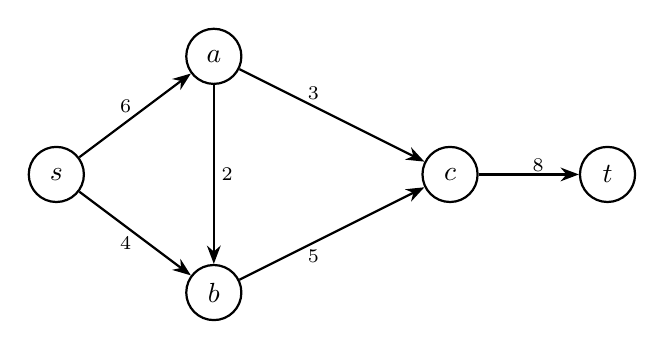
\begin{tikzpicture}[every node/.style={circle, draw, minimum size=7mm,
  inner sep=0pt}, >=Stealth, thick]
  \node (s) at (0, 0)    {$s$};
  \node (a) at (2, 1.5)  {$a$};
  \node (b) at (2, -1.5) {$b$};
  \node (c) at (5, 0)    {$c$};
  \node (t) at (7, 0)    {$t$};
  \draw[->] (s) -- node[lbl, above left]  {$6$} (a);
  \draw[->] (s) -- node[lbl, below left]  {$4$} (b);
  \draw[->] (a) -- node[lbl, above, pos=0.4] {$3$} (c);
  \draw[->] (a) -- node[lbl, right]       {$2$} (b);
  \draw[->] (b) -- node[lbl, below, pos=0.4] {$5$} (c);
  \draw[->] (c) -- node[lbl, above right] {$8$} (t);
\end{tikzpicture}
\end{center}

\vspace{8cm}

After the algorithm terminates:
\begin{enumerate}
  \item[(a)] What is the maximum flow value?
  \item[(b)] Identify the minimum cut $(S^*,\, T^*)$.  Verify
        that its capacity equals the maximum flow.
\end{enumerate}

\vfill
\newpage

% =====================================================================
% PROBLEM 4
% =====================================================================
\textbf{Problem 4.}
In the network below, a flow of value~4 has been established.
The residual graph is shown (solid = forward edges with residual
capacity, dashed = backward edges).

\begin{center}
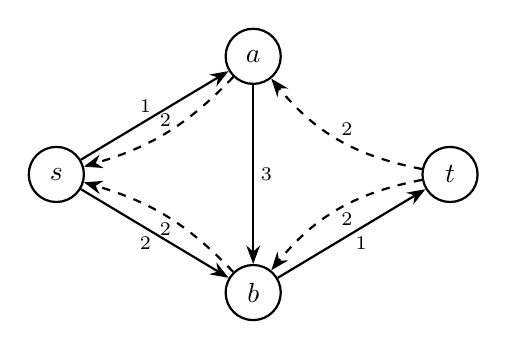
\begin{tikzpicture}[every node/.style={circle, draw, minimum size=7mm,
  inner sep=0pt}, >=Stealth, thick]
  \node (s) at (0, 0)    {$s$};
  \node (a) at (2.5, 1.5)  {$a$};
  \node (b) at (2.5, -1.5) {$b$};
  \node (t) at (5, 0)    {$t$};
  % Forward edges
  \draw[->] (s) -- node[lbl, above left]  {$1$} (a);
  \draw[->] (s) -- node[lbl, below left]  {$2$} (b);
  \draw[->] (a) -- node[lbl, right]       {$3$} (b);
  \draw[->] (b) -- node[lbl, below right] {$1$} (t);
  % Backward edges
  \draw[->, dashed] (a) to[bend left=15]
    node[lbl, above] {$2$} (s);
  \draw[->, dashed] (b) to[bend right=15]
    node[lbl, below] {$2$} (s);
  \draw[->, dashed] (t) to[bend left=20]
    node[lbl, above right] {$2$} (a);
  \draw[->, dashed] (t) to[bend right=20]
    node[lbl, below right] {$2$} (b);
\end{tikzpicture}
\end{center}

\begin{enumerate}
  \item[(a)] Can you find an augmenting $s \to t$ path in this
        residual graph?  If so, how much flow can you push?

  \vspace{3.5cm}

  \item[(b)] If no augmenting path exists, identify the set
        $S^*$ of vertices reachable from $s$ in the residual
        graph.  What is the minimum cut?

  \vspace{3.5cm}

  \item[(c)] Verify that $v(f) = c(S^*, V \setminus S^*)$.
\end{enumerate}

\vfill
\end{document}
